\documentclass[12pt]{article}

\usepackage{answers}
\usepackage{setspace}
\usepackage{graphicx}
\usepackage{enumitem}
\usepackage{multicol}
\usepackage{mathrsfs}
\usepackage[margin=1in]{geometry} 
\usepackage{amsmath,amsthm,amssymb}
 \usepackage{graphicx}
 \usepackage{epstopdf} %%package to overcome problem with eps in pdf files
 \usepackage{float}
 
\newcommand{\N}{\mathbb{N}}
\newcommand{\Z}{\mathbb{Z}}
\newcommand{\C}{\mathbb{C}}
\newcommand{\R}{\mathbb{R}}

\DeclareMathOperator{\sech}{sech}
\DeclareMathOperator{\csch}{csch}
 
\newenvironment{theorem}[2][Theorem]{\begin{trivlist}
\item[\hskip \labelsep {\bfseries #1}\hskip \labelsep {\bfseries #2.}]}{\end{trivlist}}
\newenvironment{definition}[2][Definition]{\begin{trivlist}
\item[\hskip \labelsep {\bfseries #1}\hskip \labelsep {\bfseries #2.}]}{\end{trivlist}}
\newenvironment{proposition}[2][Proposition]{\begin{trivlist}
\item[\hskip \labelsep {\bfseries #1}\hskip \labelsep {\bfseries #2.}]}{\end{trivlist}}
\newenvironment{lemma}[2][Lemma]{\begin{trivlist}
\item[\hskip \labelsep {\bfseries #1}\hskip \labelsep {\bfseries #2.}]}{\end{trivlist}}
\newenvironment{exercise}[2][Exercise]{\begin{trivlist}
\item[\hskip \labelsep {\bfseries #1}\hskip \labelsep {\bfseries #2.}]}{\end{trivlist}}
\newenvironment{solution}[2][Solution]{\begin{trivlist}
\item[\hskip \labelsep {\bfseries #1}]}{\end{trivlist}}
\newenvironment{problem}[2][Problem]{\begin{trivlist}
\item[\hskip \labelsep {\bfseries #1}\hskip \labelsep {\bfseries #2.}]}{\end{trivlist}}
\newenvironment{question}[2][Question]{\begin{trivlist}
\item[\hskip \labelsep {\bfseries #1}\hskip \labelsep {\bfseries #2.}]}{\end{trivlist}}
\newenvironment{corollary}[2][Corollary]{\begin{trivlist}
\item[\hskip \labelsep {\bfseries #1}\hskip \labelsep {\bfseries #2.}]}{\end{trivlist}}
 
\begin{document}
 
% --------------------------------------------------------------
%                         Start here
% --------------------------------------------------------------
 
\title{Assignment 2}%replace with the appropriate homework number
\author{2019701007\\ %replace with your name
SMAI-M-19} %if necessary, replace with your course title
 
\maketitle
%Below is an example of the problem environment

\begin{problem}{1}
	\
	\begin{enumerate}[label=\alph*)]
		\item What are eigen faces?
		\\
		The eigenvectors which we derive from the covariance matrix of faces, and then those eigenvectors are called as eigenfaces. And any face is then some linear combination of those eigen faces. Eigen faces are blurry depiction of faces, each one highlighting certain type of features.
		\item How many eigen vec-tors/faces are required to “satisfactorily” reconstruct a person in these three datasets?
		\\
		Based on the eigen spectrum, if we need about 80-85 \% variance in the data, For the yale dataset we need about 10 Eigen Faces, as it is Grayscale image. For IMFDB dataset, we need about 25 EigenFaces, as it is RGB. For IIIT-CFW, its RGB image, plus there is lot of different pattern in data, its really hard to learn from it. so we would need about 40-50 eigenfaces minimum. 
		\begin{figure}[H]
			\centering
			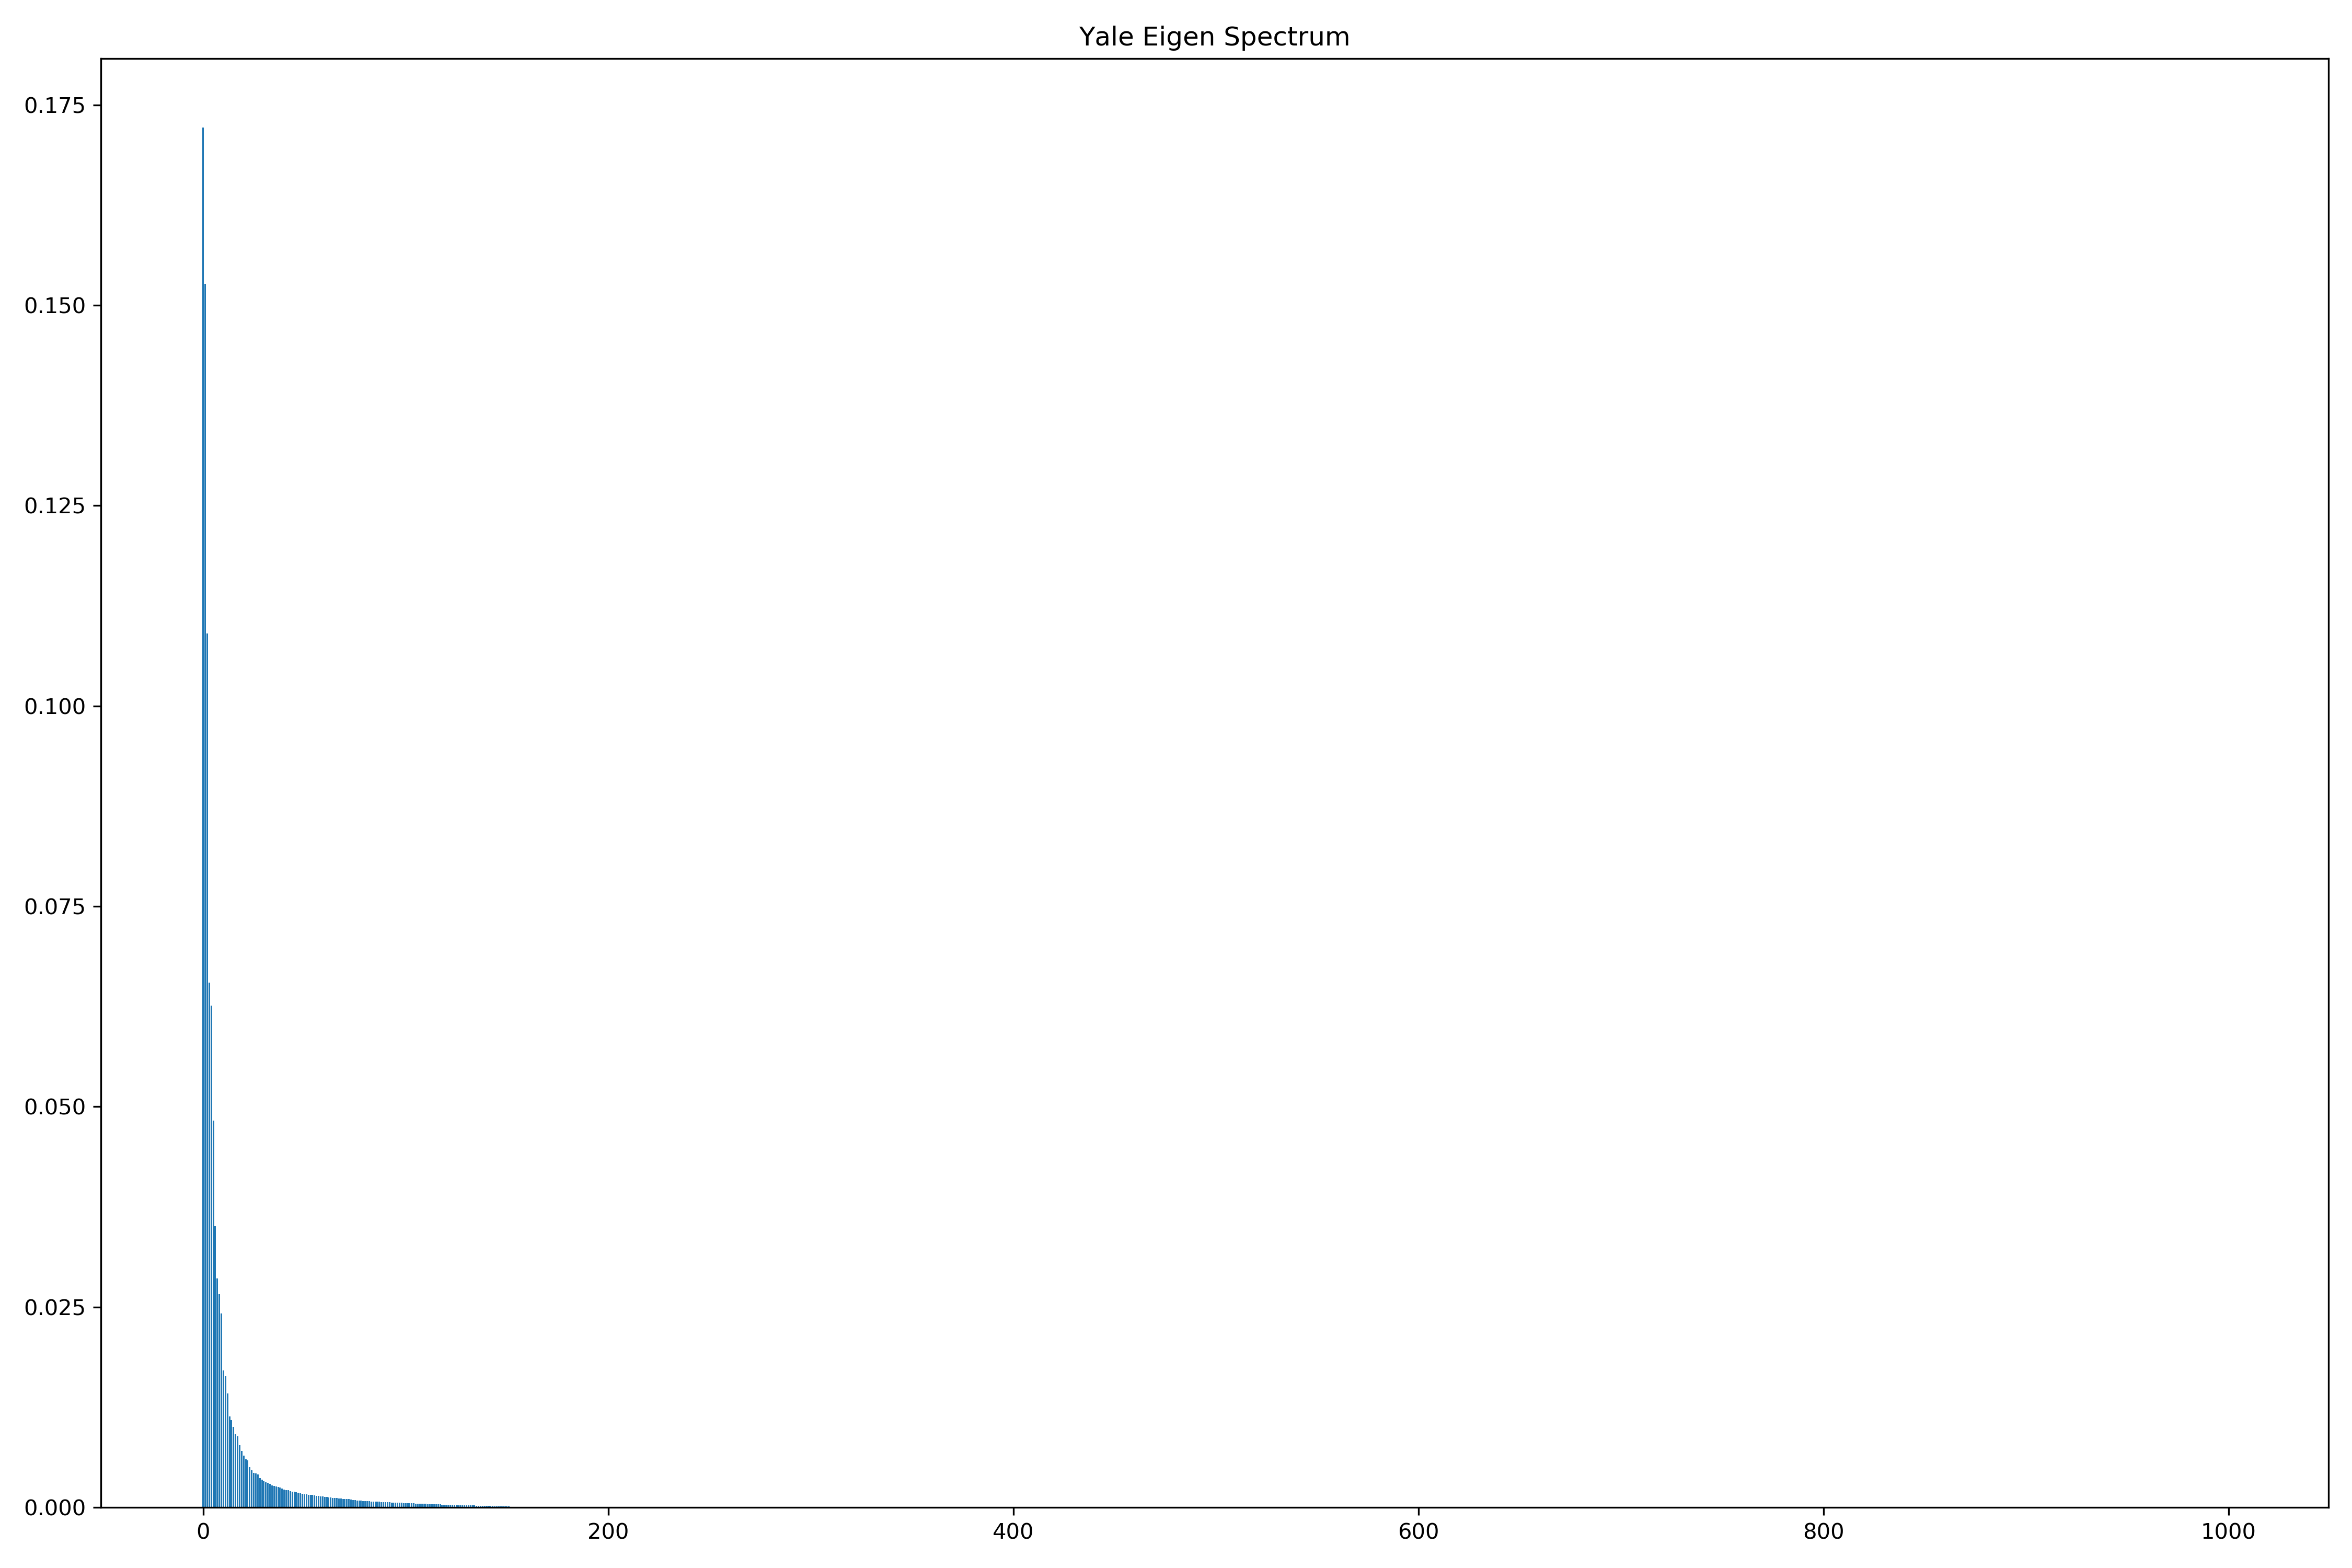
\includegraphics[totalheight=8cm]{Yale_Eigen_Spectrum.png}
			\caption{Yale Eigen Spectrum}
			\label{fig:verticalcell}
		\end{figure}
		
		\begin{figure}[H]
			\centering
			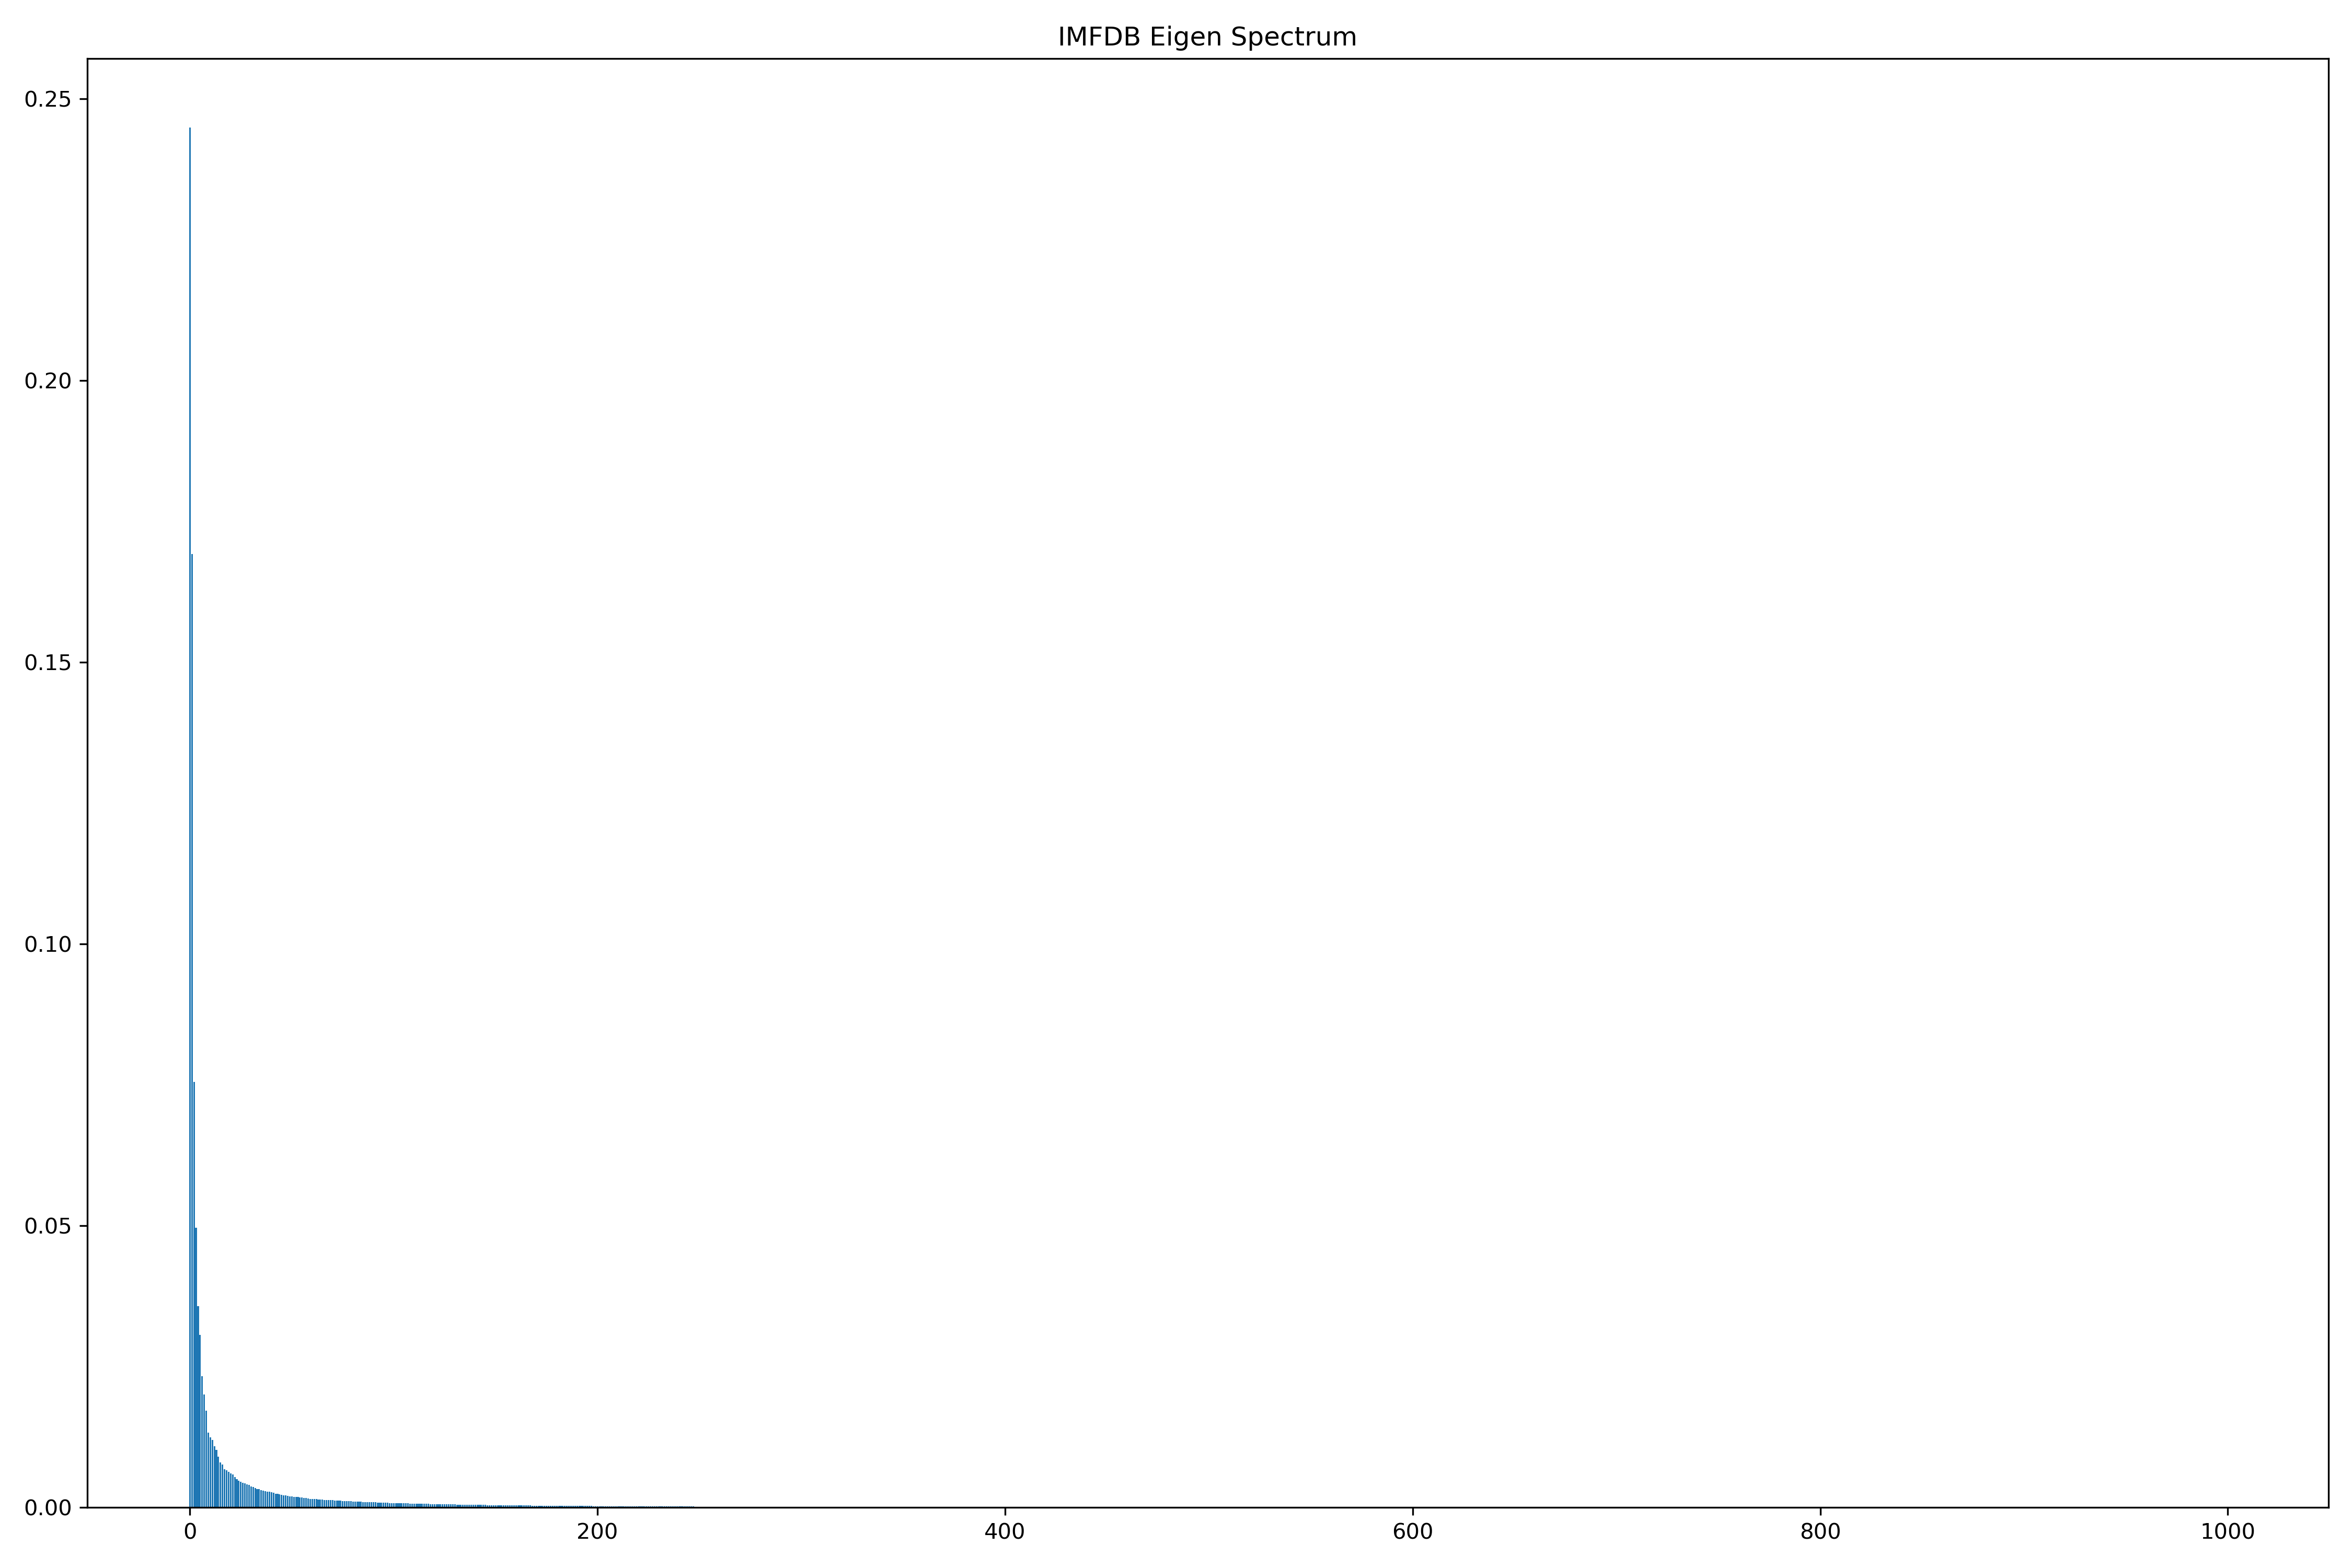
\includegraphics[totalheight=8cm]{IMFDB_Eigen_Spectrum.png}
			\caption{IMFDB Eigen Spectrum}
			\label{fig:verticalcell}
		\end{figure}
		
		\begin{figure}[H]
			\centering
			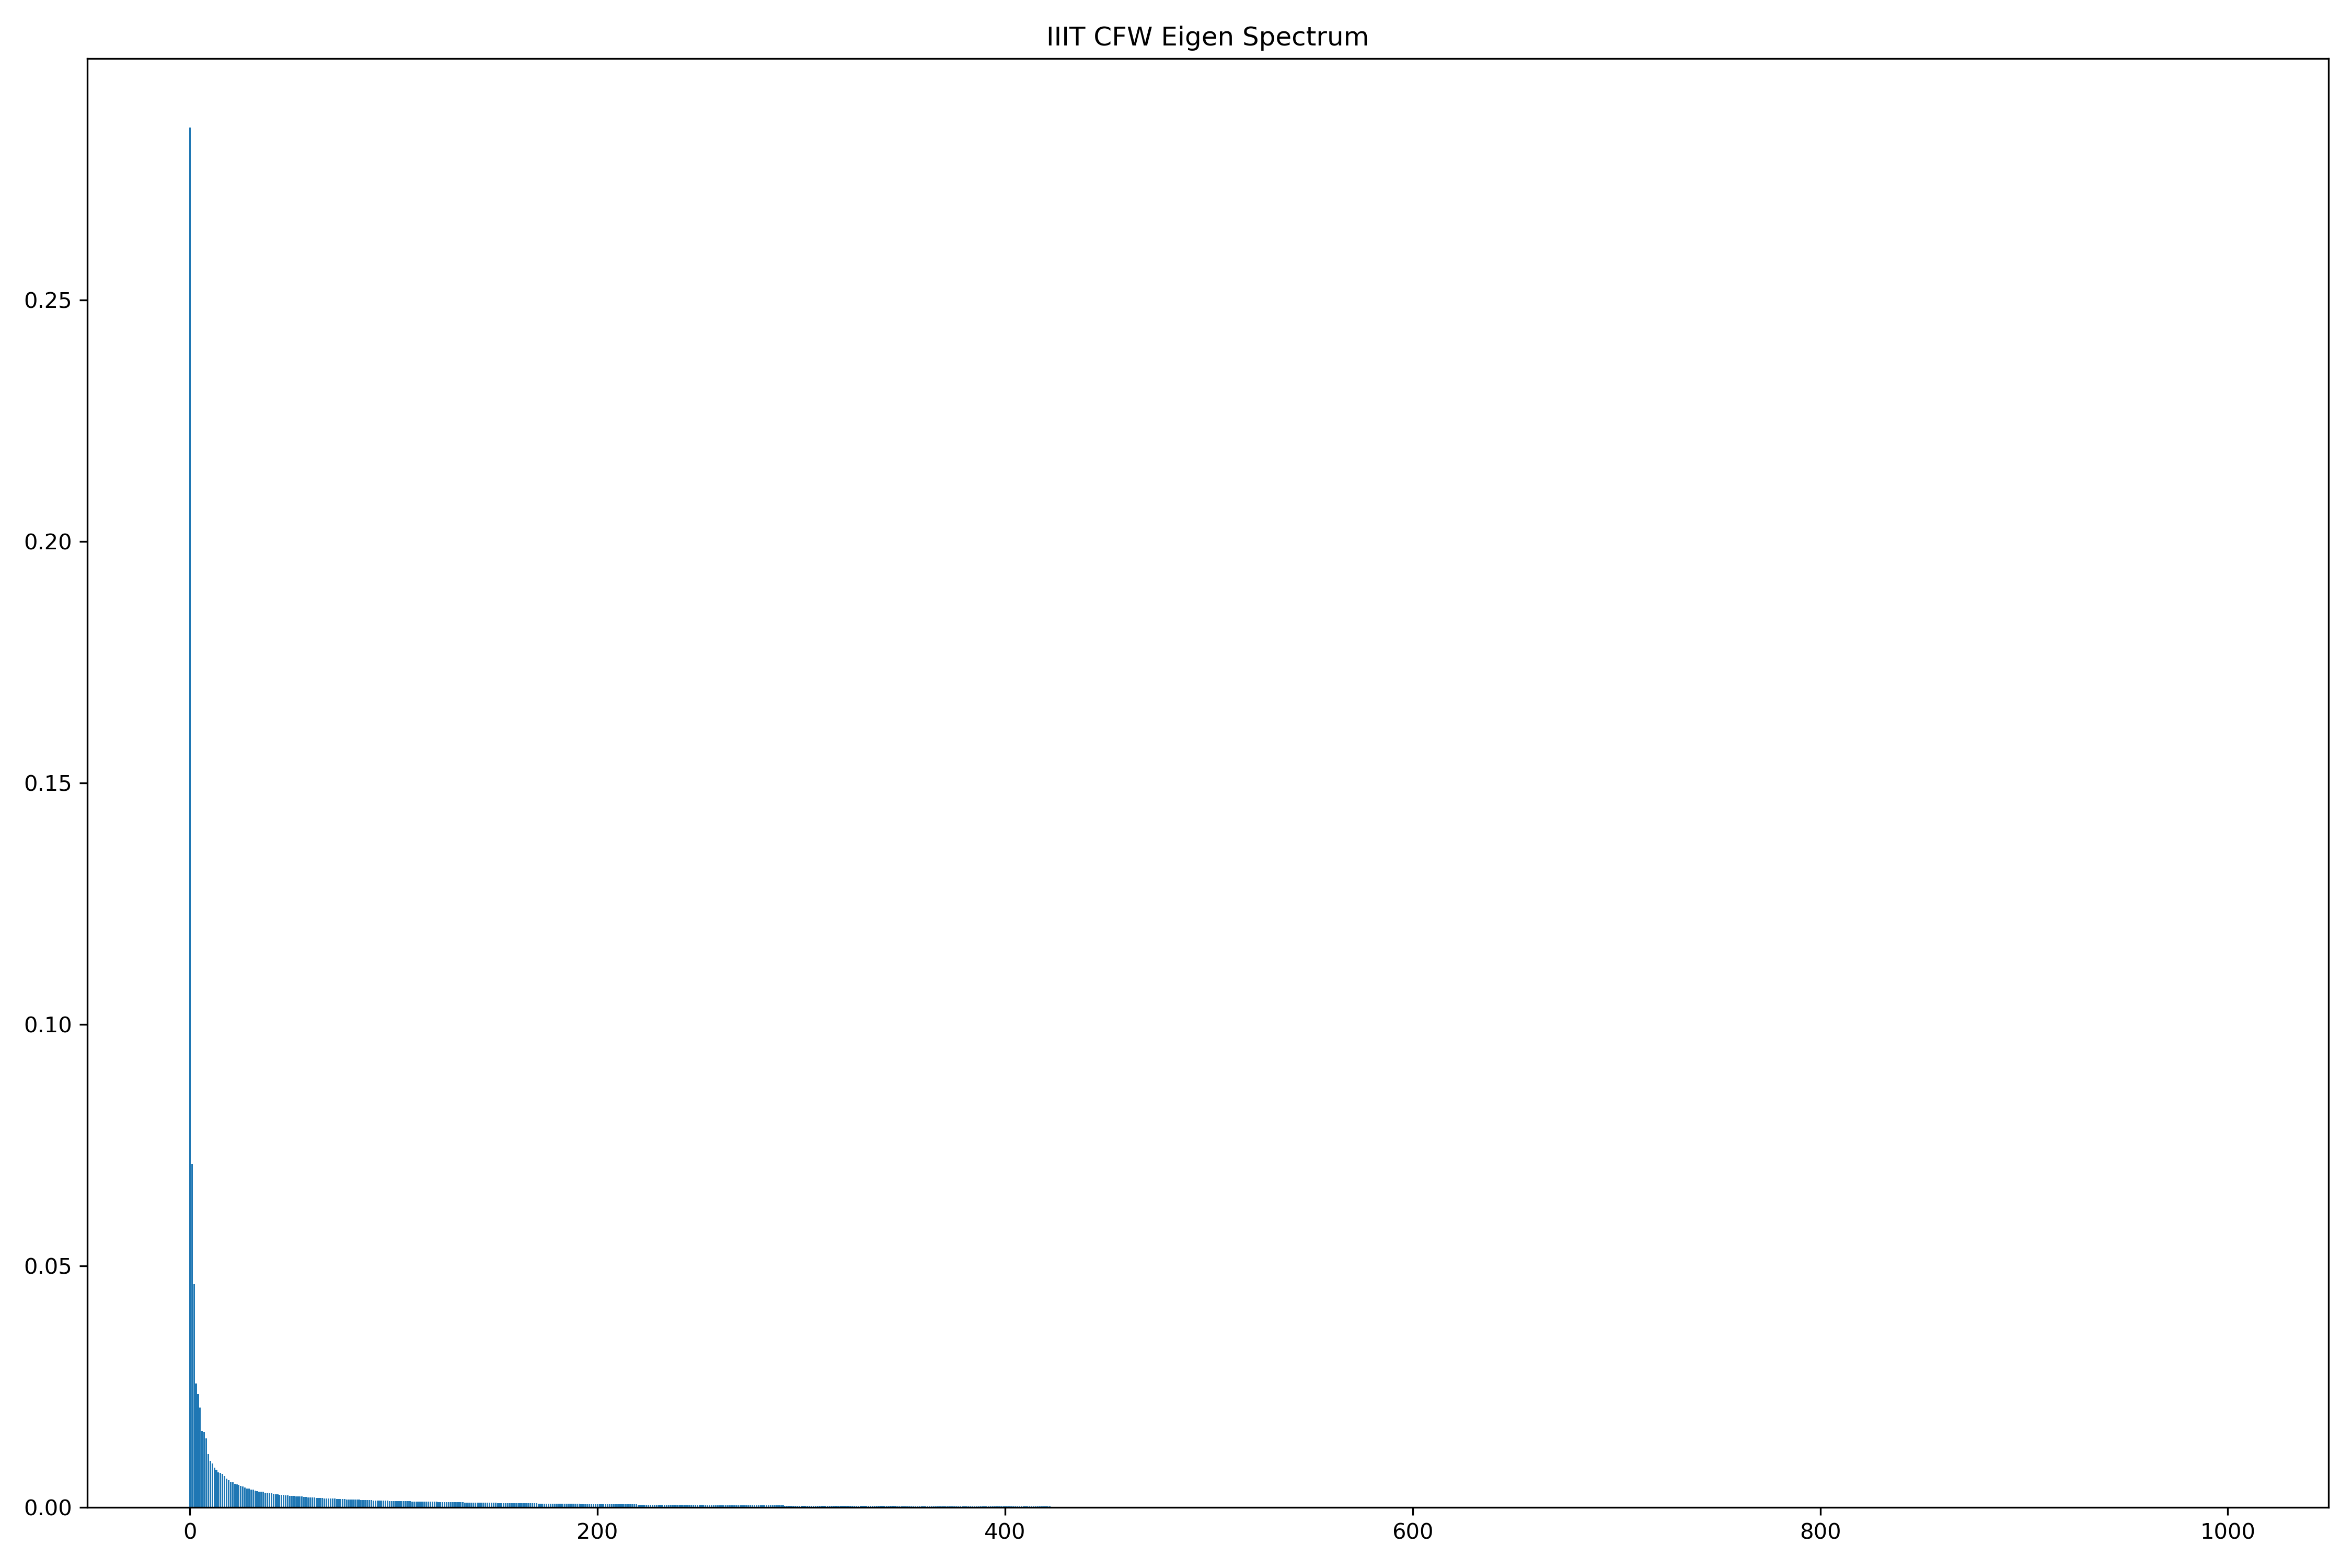
\includegraphics[totalheight=8cm]{IIIT_CFW_Eigen_Spectrum.png}
			\caption{IIIT CFW Eigen Spectrum}
			\label{fig:verticalcell}
		\end{figure}
		
		
		\item Reconstruct the image back for each case
		Plotting randomly taken 6 faces for each dataset. 
		
		\begin{figure}[H]
			\centering
			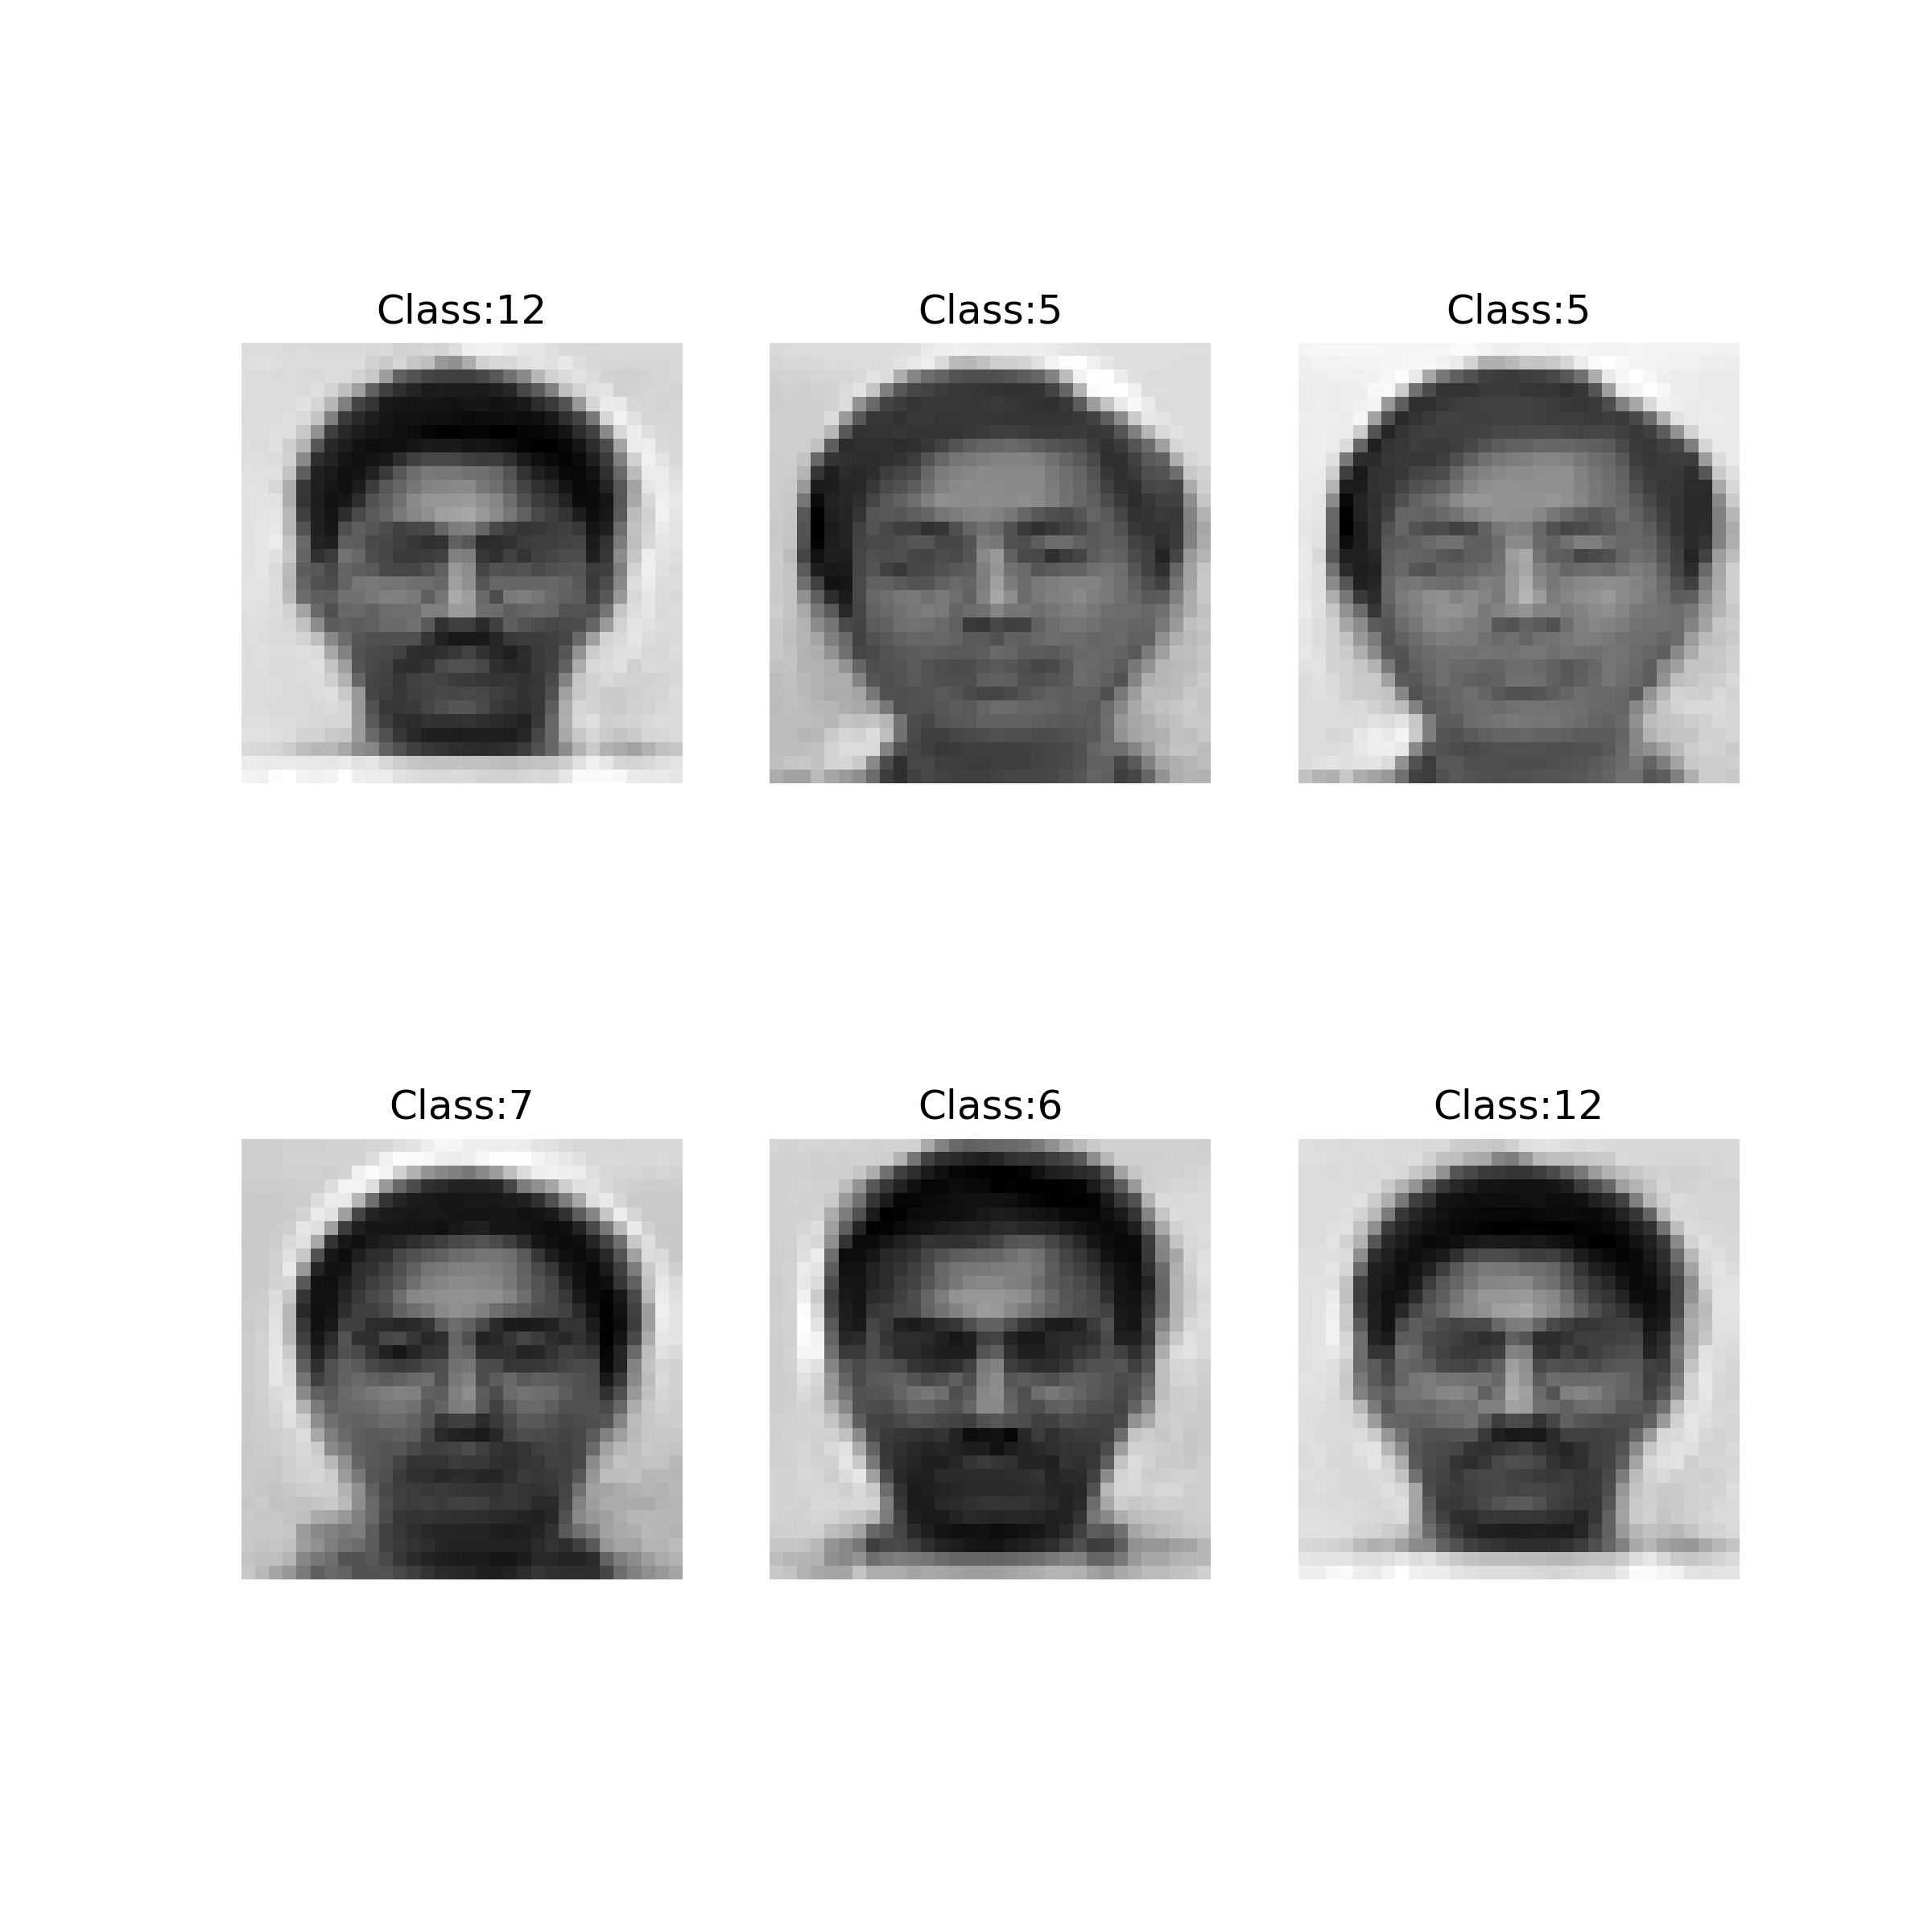
\includegraphics[totalheight=8cm]{Reconstruction_For_Yale_Face_Database.png}
			\caption{Reconstruction For Yale Face Database}
			\label{fig:verticalcell}
		\end{figure}
		
		\begin{figure}[H]
			\centering
			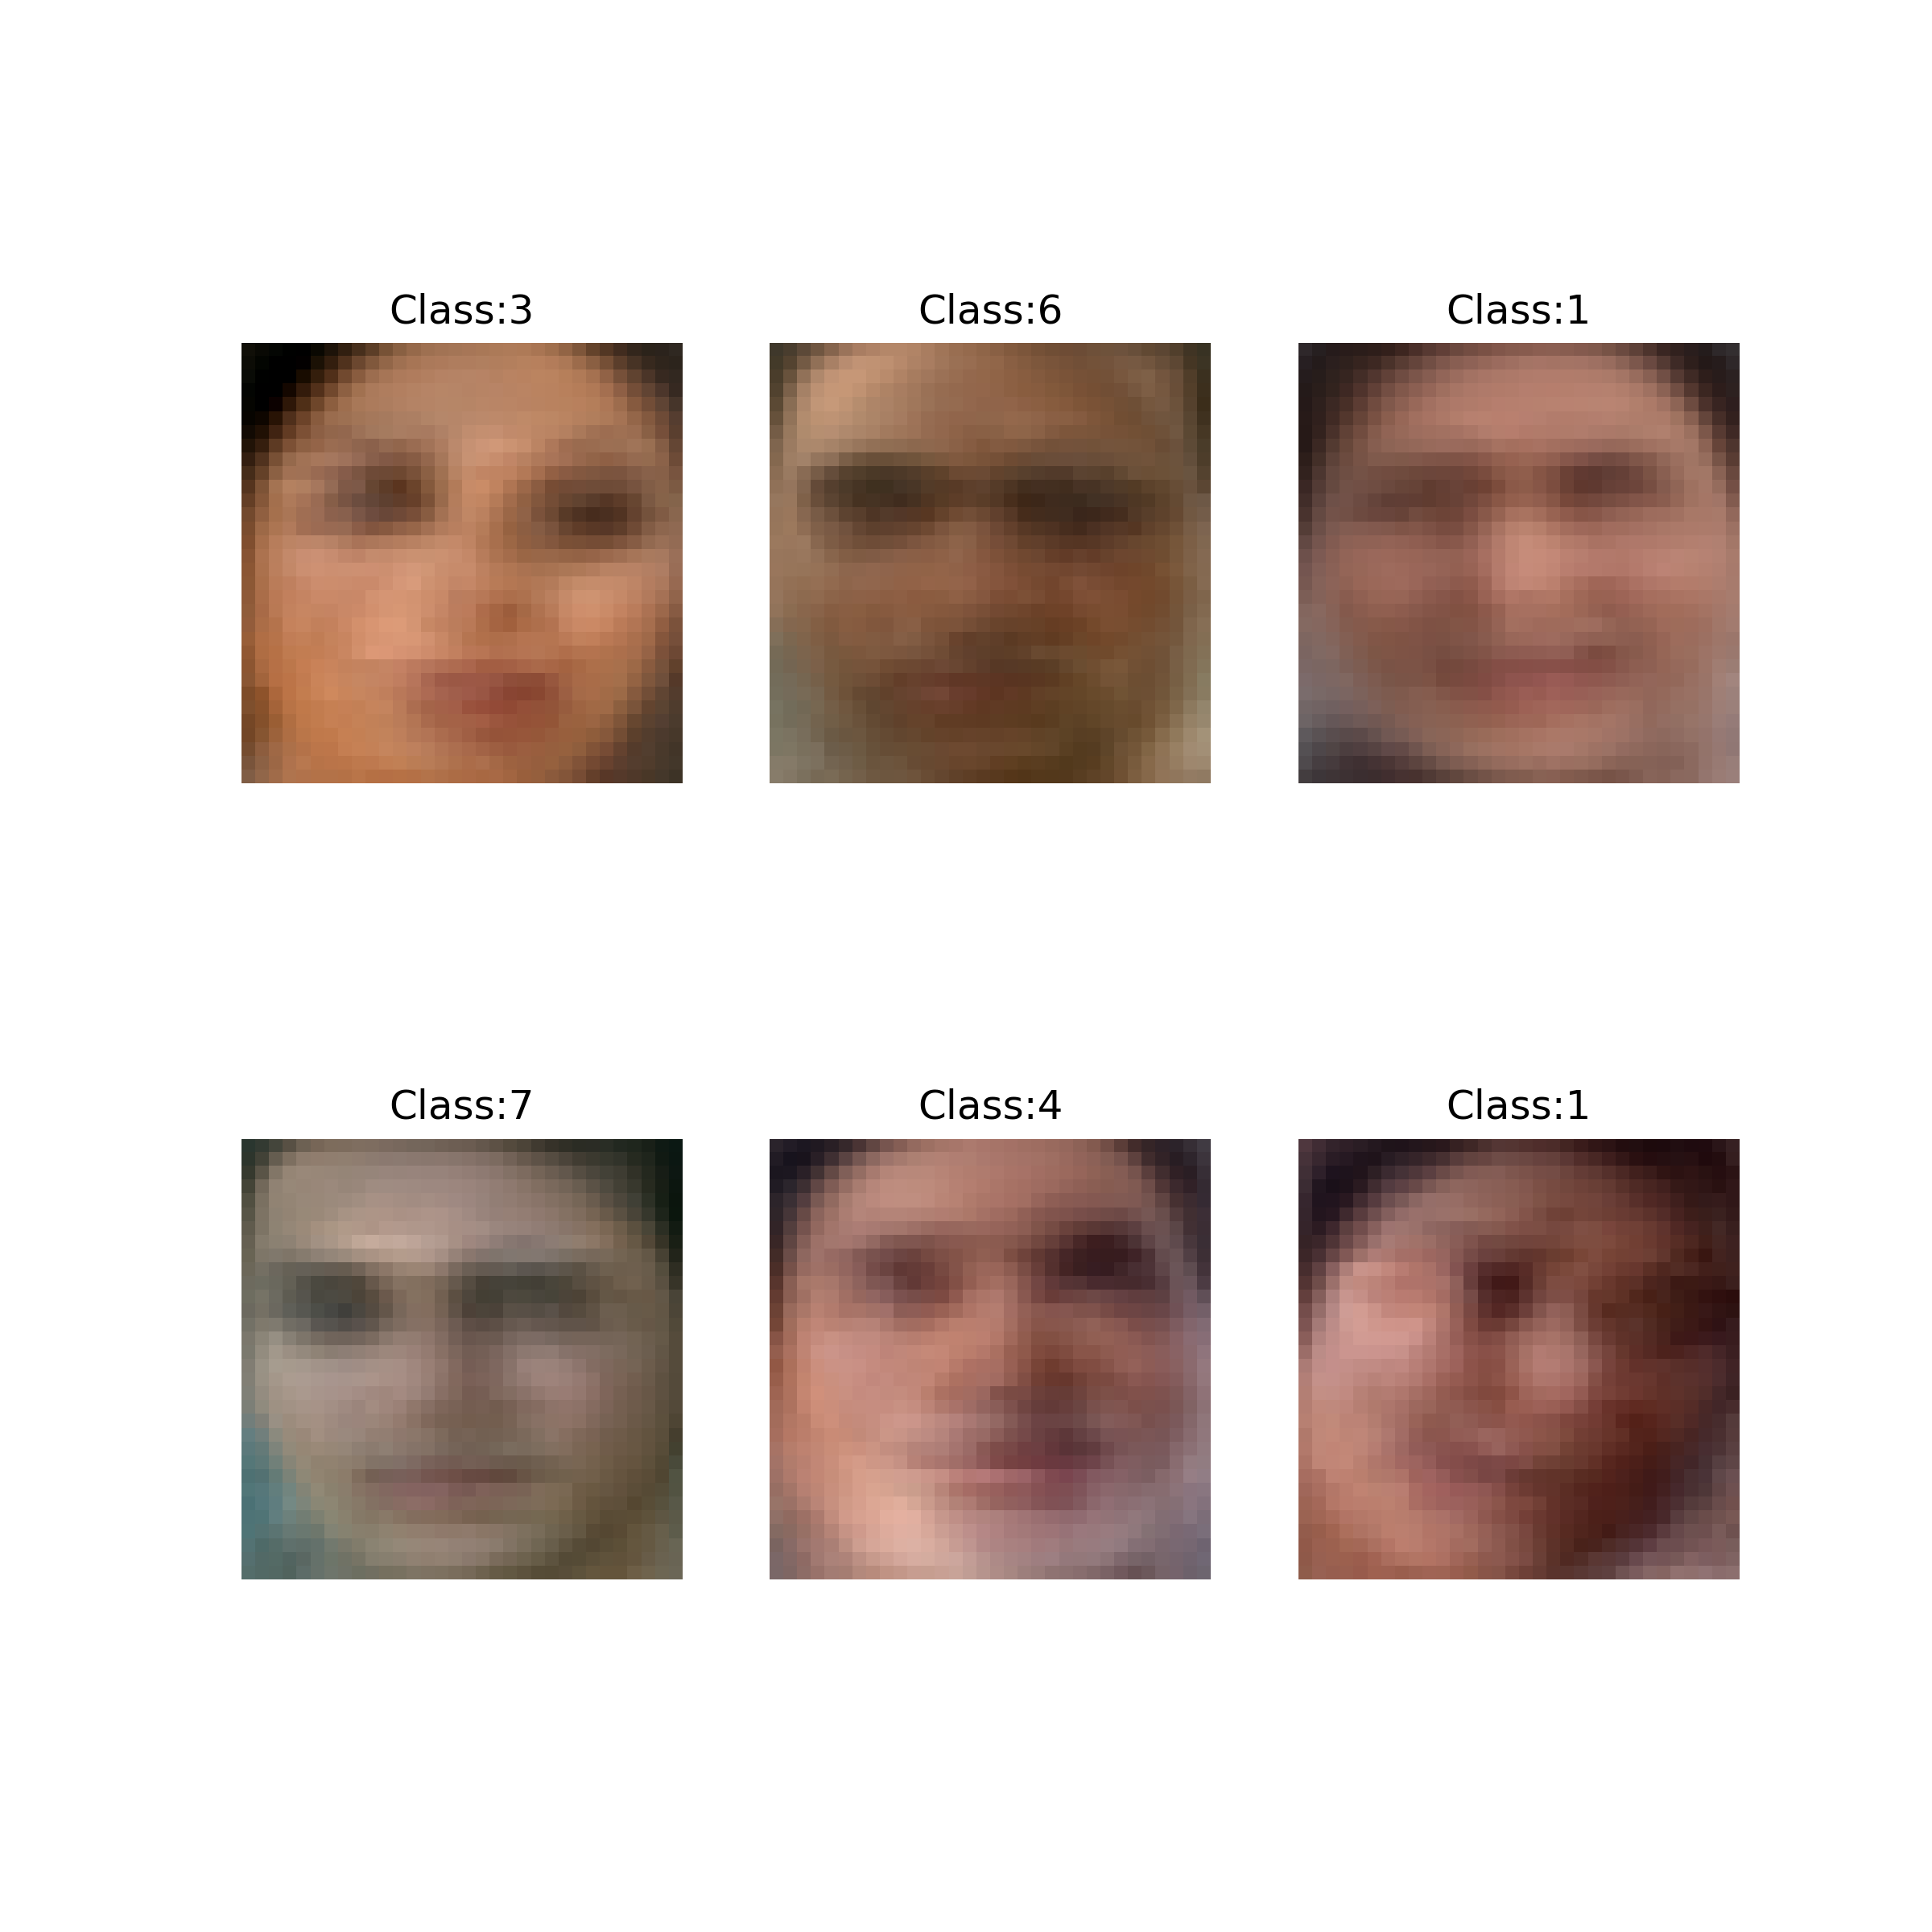
\includegraphics[totalheight=8cm]{Reconstruction_For_IMFDB_Database.png}
			\caption{Reconstruction For IMFDB Database}
			\label{fig:verticalcell}
		\end{figure}
		
		\begin{figure}[H]
			\centering
			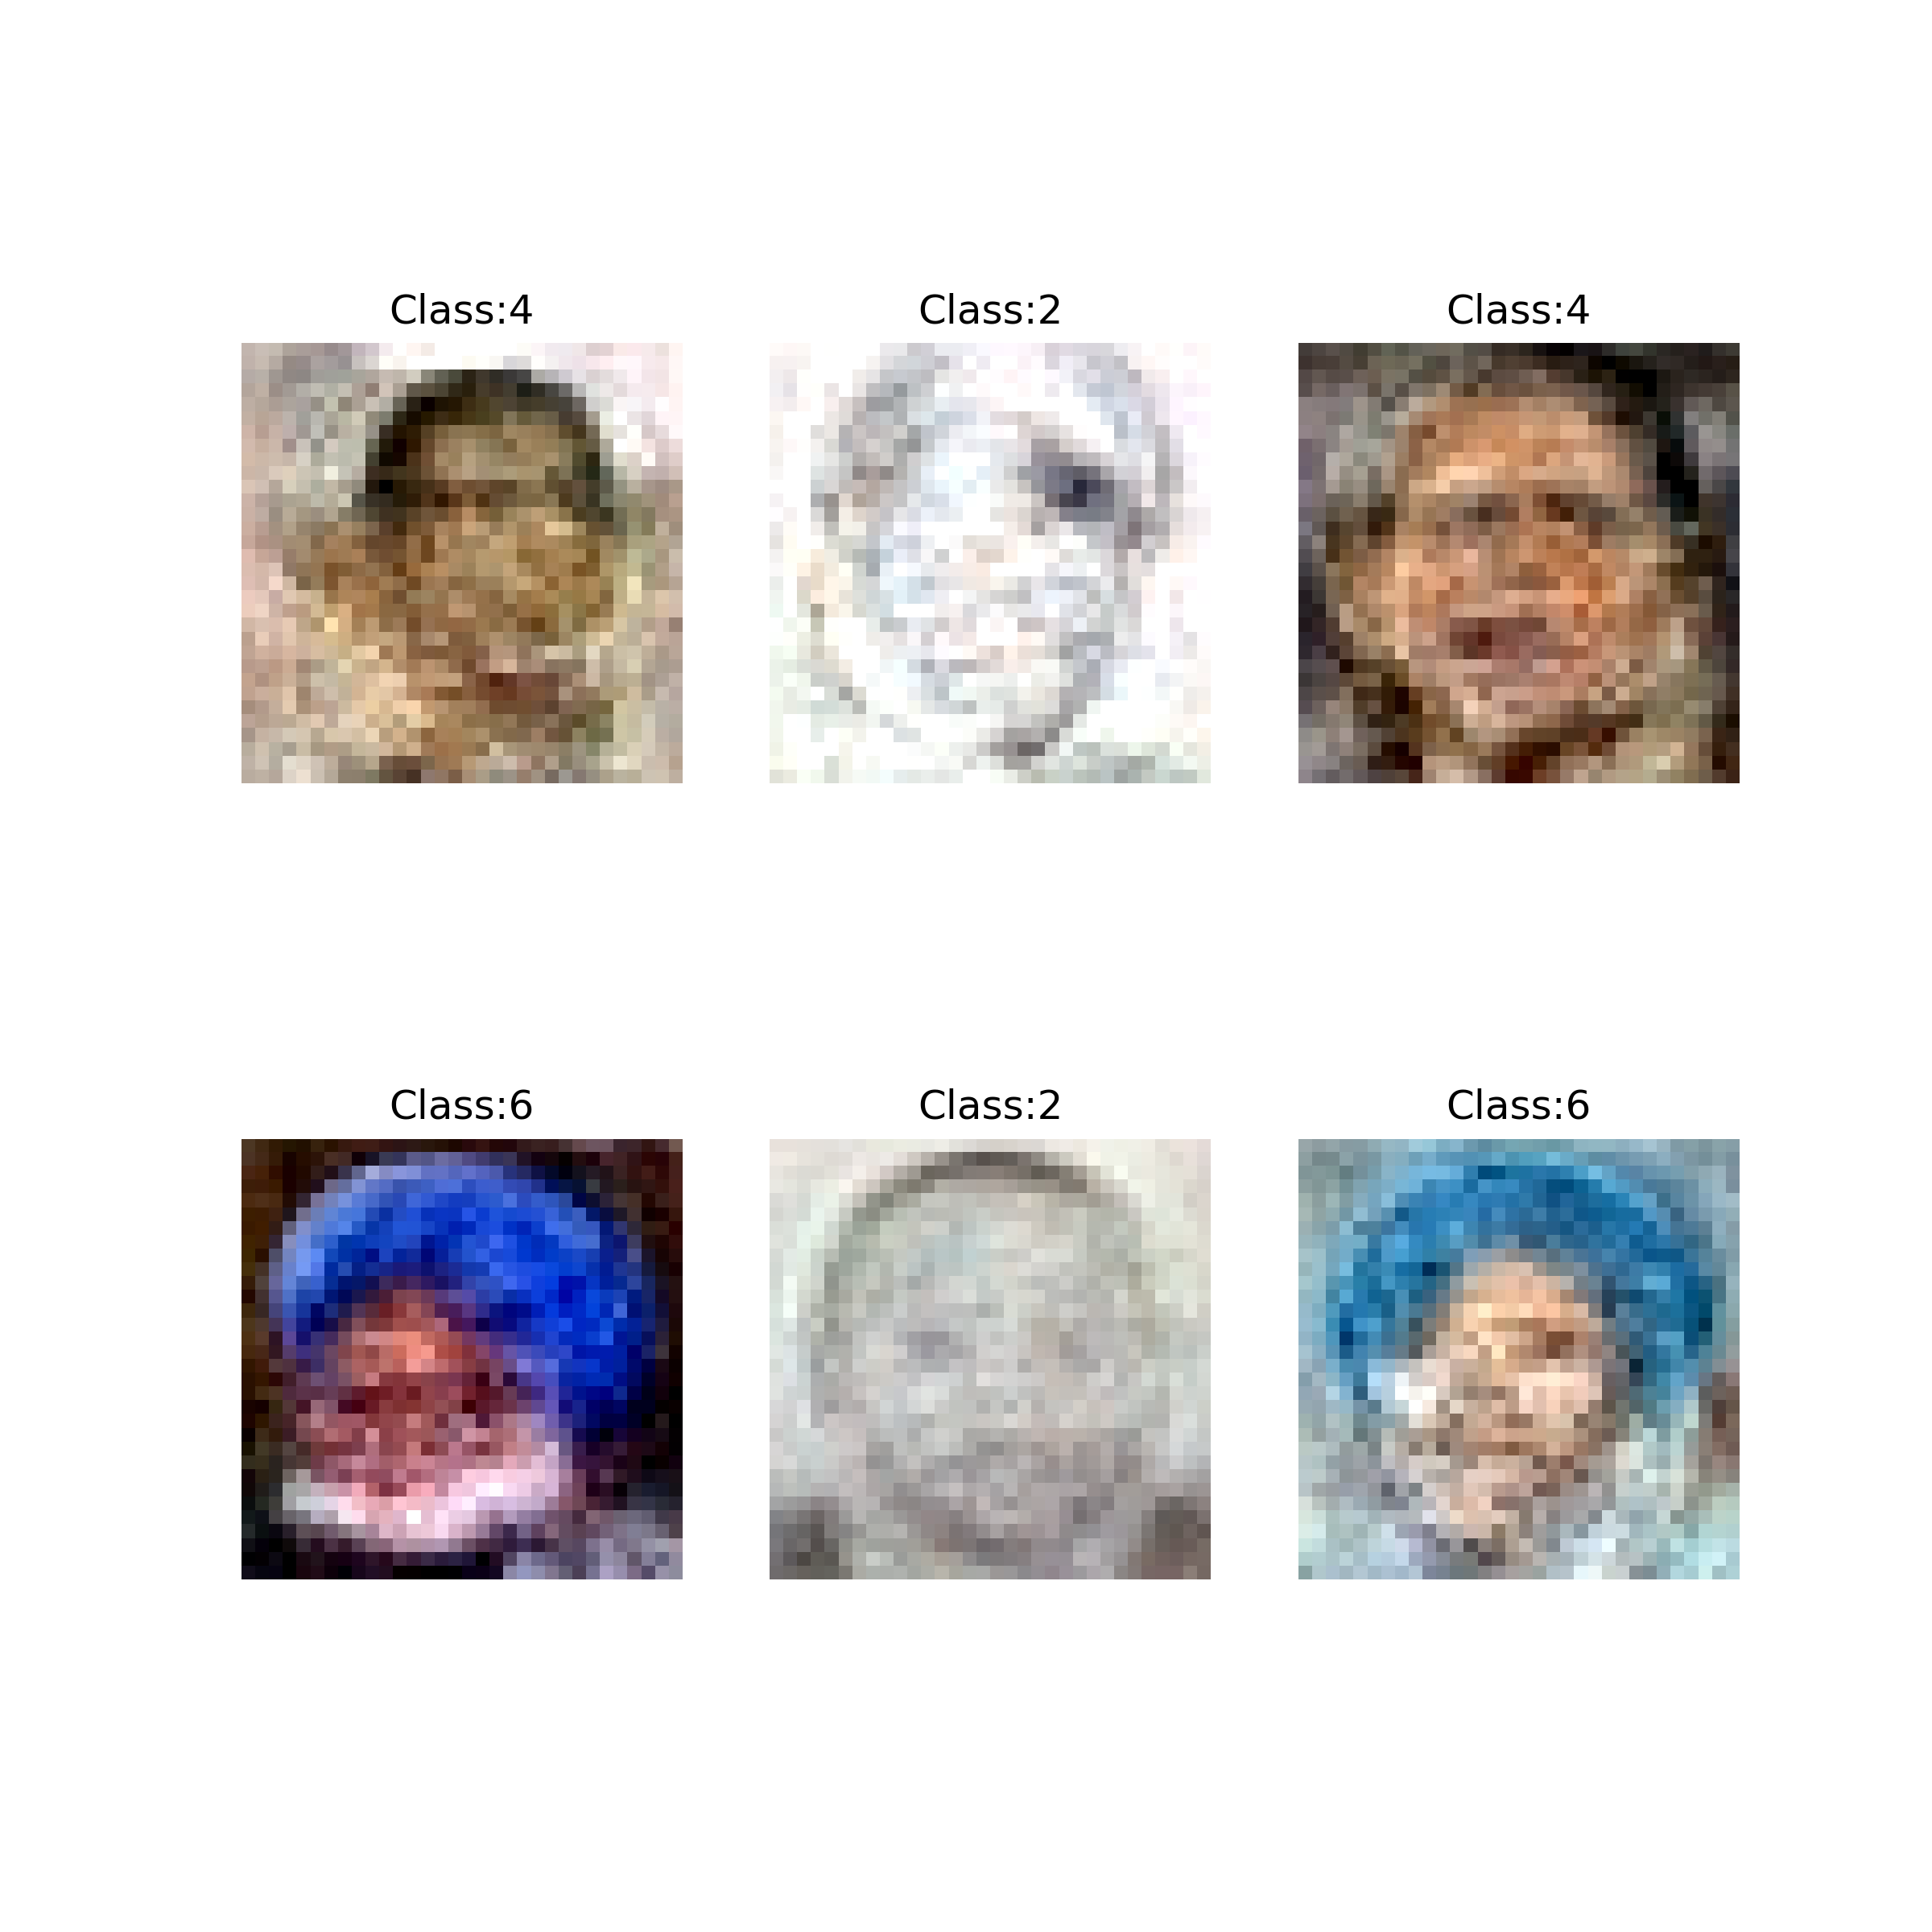
\includegraphics[totalheight=8cm]{Reconstruction_For_IIIT_CFW_Database.png}
			\caption{Reconstruction For IIIT - CFW Database}
			\label{fig:verticalcell}
		\end{figure}
		
		
		\item Which person/identity is difficult to represent com-pactly with fewer eigen vectors? Why is that? Explain with your empirical observations and intuitive answers
	\end{enumerate}
\end{problem}

\begin{problem}{2}
	Use an MLP classifier and find the classification accuracy. Which method works well? Do a comparitive
	study.
	\\
	From the emperical results, for each dataset, LDA, Kernel LDA and Resnet features are doing much better. And in comparision, LDA and Kernel LDA are doing the most dimensional reduction and giving much higher accuracy. Even on the tough dataset like IIIT - CFW. 
	
	
			\begin{figure}[H]
		\centering
		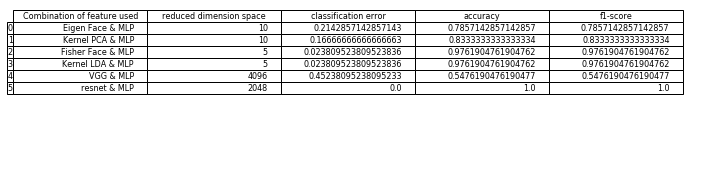
\includegraphics[width=16cm]{Yale_Face_Classification_Feature_Comparision.png}
		\caption{Yale Face Classification - Feature Comparision}
		\label{fig:verticalcell}
	\end{figure}
	
	
	\begin{figure}[H]
		\centering
		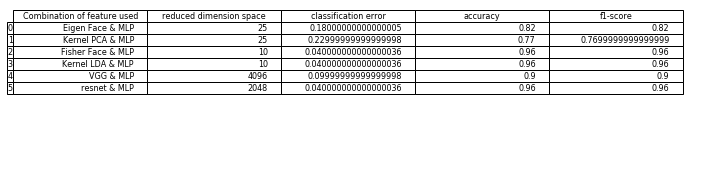
\includegraphics[width=16cm]{IMFDB_Face_Classification_Feature_Comparision.png}
		\caption{IMFDB Face Classification - Feature Comparision}
		\label{fig:verticalcell}
	\end{figure}


	
	\begin{figure}[H]
		\centering
		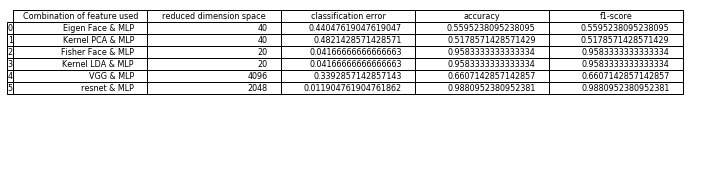
\includegraphics[width=16cm]{IIIT_CFW_Face_Classification_Feature_Comparision.png}
		\caption{IIIT-CFW Face Classification - Feature Comparision}
		\label{fig:verticalcell}
	\end{figure}
	
\end{problem}


\begin{problem}{3}
Use t-SNE based visilization of faces? Does it make
sense? Do you see similar people coming together?
or something else? Can you do visualization dataset
wise and combined?
	\\It doesn't show a nice classification like we get in PCA or LDA with 2 or 3 dimensions. Everything looks mixed	
		\begin{figure}[H]
		\centering
		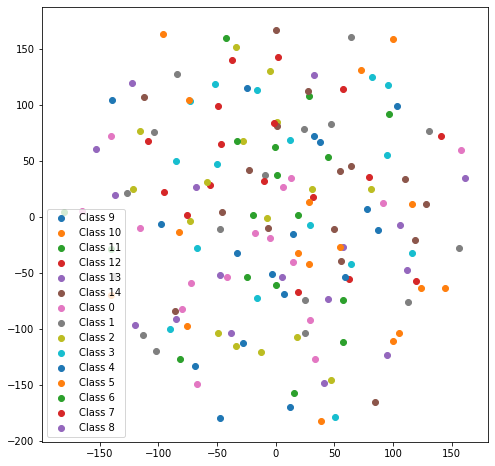
\includegraphics[width=16cm]{Yale_Database_with_2_Components.png}
		\caption{Yale Database with 2 Components}
		\label{fig:verticalcell}
	\end{figure}
	
	
		\begin{figure}[H]
		\centering
		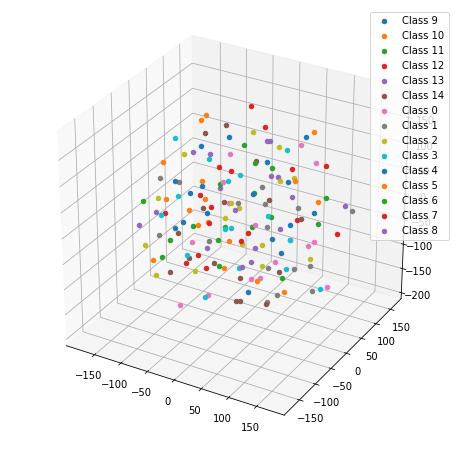
\includegraphics[width=16cm]{Yale_Database_with_3_Components.png}
		\caption{Yale Database with 3 Components}
		\label{fig:verticalcell}
	\end{figure}
	
	
		\begin{figure}[H]
		\centering
		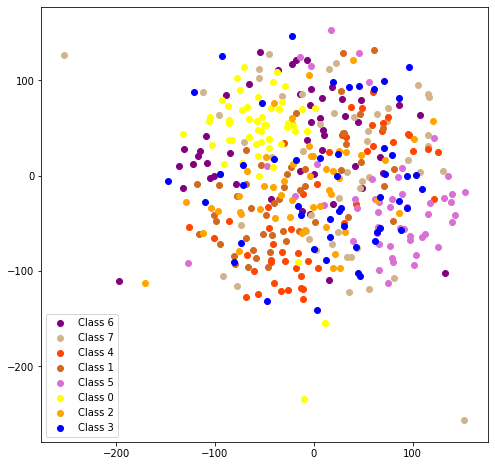
\includegraphics[width=16cm]{IMFDB_Database_with_2_Components.png}
		\caption{IMFDB Database with 2 Components}
	%	\label{fig:verticalcell}
	\end{figure}
	
	
	\begin{figure}[H]
		\centering
		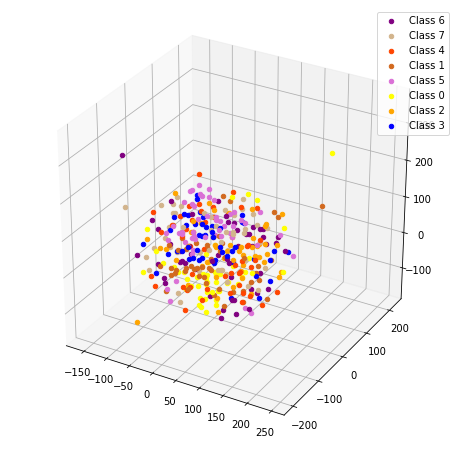
\includegraphics[width=16cm]{IMFDB_Database_with_3_Components.png}
		\caption{IMFDB Database with 3 Components}
	%	\label{fig:verticalcell}
	\end{figure}
	
	\begin{figure}[H]
		\centering
		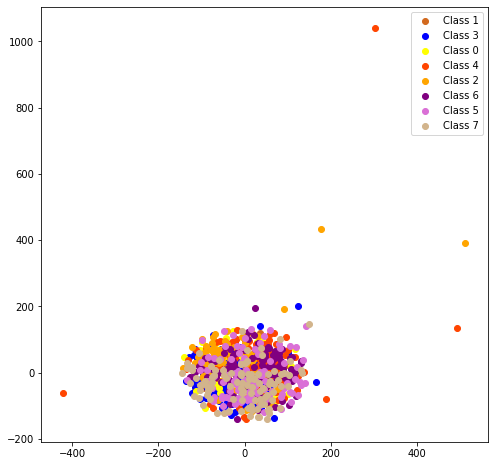
\includegraphics[width=16cm]{IIIT_CFW_Database_with_2_Components.png}
		\caption{IIIT-CFW Database with 2 Components}
		%	\label{fig:verticalcell}
	\end{figure}
	
	
	\begin{figure}[H]
		\centering
		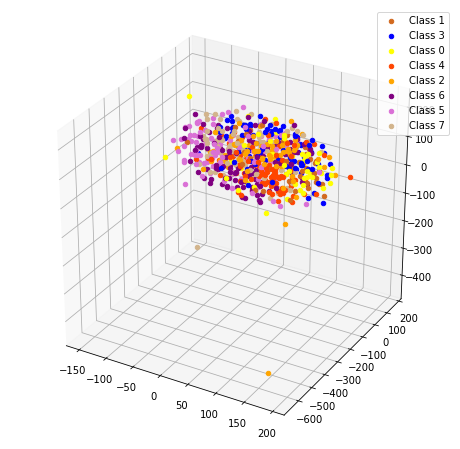
\includegraphics[width=16cm]{IIIT_CFW_Database_with_3_Components.png}
		\caption{IIIT-CFW Database with 3 Components}
		%	\label{fig:verticalcell}
	\end{figure}
	

\begin{figure}[H]
	\centering
	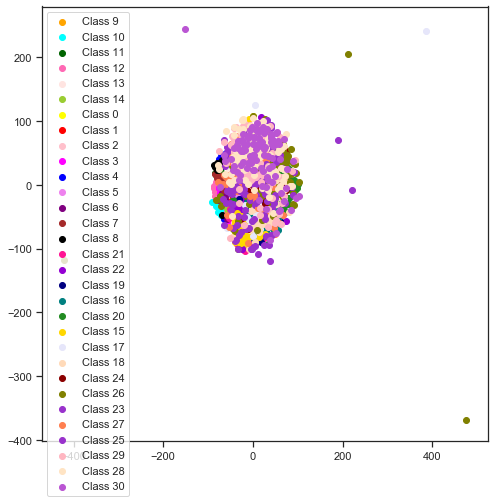
\includegraphics[width=16cm]{Combined_Database_with_2_Components.png}
	\caption{Combined Database with 2 Components}
	%	\label{fig:verticalcell}
\end{figure}


\begin{figure}[H]
	\centering
	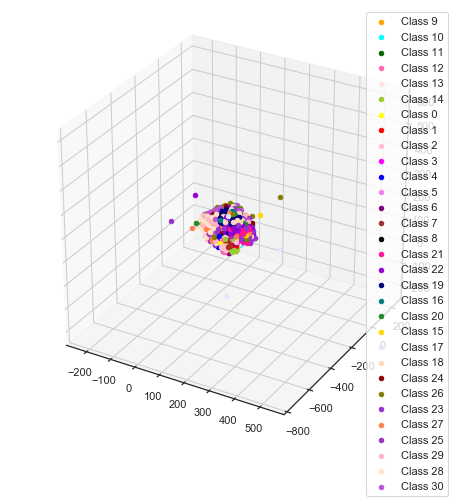
\includegraphics[width=16cm]{Combined_Database_with_3_Components.png}
	\caption{Combined Database with 3 Components}
	%	\label{fig:verticalcell}
\end{figure}
\end{problem}



\begin{problem}{4}
In practice "face" is used for verification. i.e., input is "identity/classID) and the face image" and
response is "Yes" or "No". (i) How do we formulate
the problem using KNN (ii) How do we analyze the
performance ? suggest the metrics (like accuracy)
that is appropriate for this task. Show empirical results with all the representations and variations in
K

	\begin{figure}[H]
		\centering
		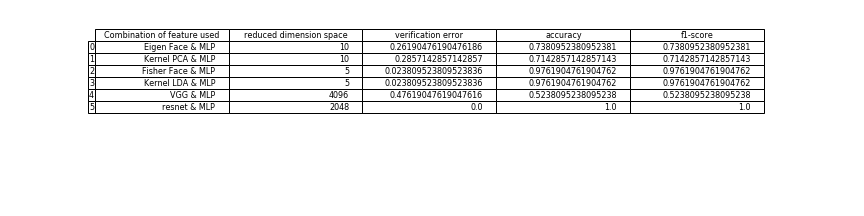
\includegraphics[width=16cm]{Yale_Face_Verification_Comparision.png}
		\caption{Yale Face Verification - Comparision}
		\label{fig:verticalcell}
	\end{figure}
	
	
	\begin{figure}[H]
		\centering
		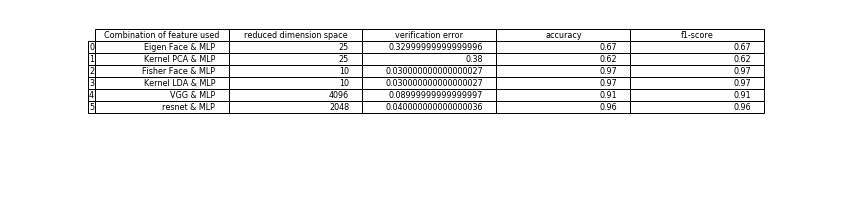
\includegraphics[width=16cm]{IMFDB_Face_Verification_Comparision.png}
		\caption{IMFDB Face Verification -  Comparision}
		%	\label{fig:verticalcell}
	\end{figure}
	
	
	\begin{figure}[H]
		\centering		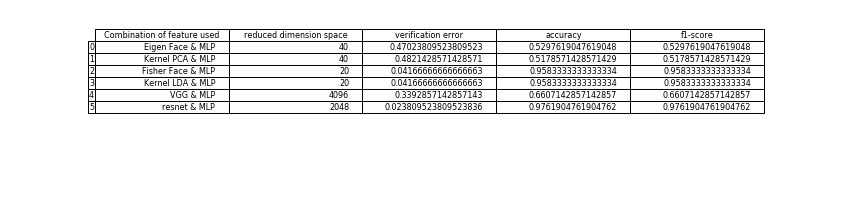
\includegraphics[width=16cm]{IIIT_CFW_Face_Verification_Comparision.png}
		\caption{IIIT-CFW Face Verification -  Comparision}
		%	\label{fig:verticalcell}
	\end{figure}
	
\end{problem}




\begin{problem}{4}
Emotion classification
Briefly explain the problem. Why the problem is not
trivial.Why a solution to this may be of some use. Suggest
good applications. Suggest good reasons why solving
your problem is. Explain your experimental pipeline, splits, evaluation metrics, quantitative results, qualitative results
\\
\\
 Doing emotion classification based on the emotion provided in emotion.txt of IMFDB and Yale Dataset.
Emotion classification can be useful for security purpose. People can rarely hide microexpression. So If we have footage of their interogation, we can apply classification, and pick out emotion which as a human we can miss.
\\ Apply MLP on LDA features, gives 90\% accuracy. It misclassified 10\%  
Precision Score is 0.9 Recall Score is 0.9
F1 Score is 0.9
\\ Plotted facetgrid for TSNE features, and scatter plot for PCA and LDA



\begin{figure}[H]
	\centering		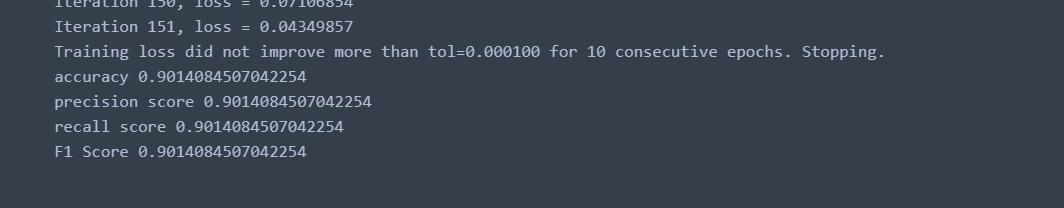
\includegraphics[width=16cm]{emotion_classification_accuracy.png}
	\caption{Metrics of classification}
	%	\label{fig:verticalcell}
\end{figure}


\begin{figure}[H]
	\centering		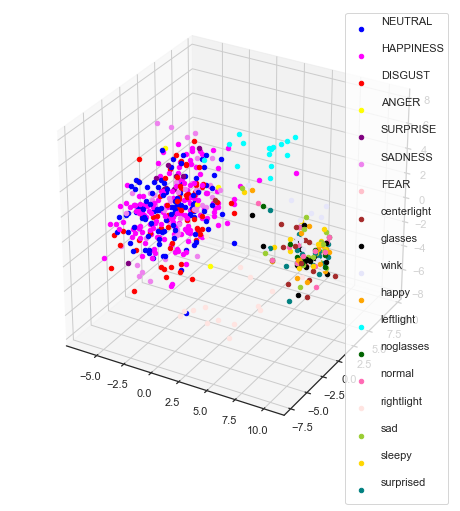
\includegraphics[width=16cm]{Scatter_Plot_of_pca.png}
	\caption{Scatter Plot of PCA Features}
	%	\label{fig:verticalcell}
\end{figure}


\begin{figure}[H]
	\centering
	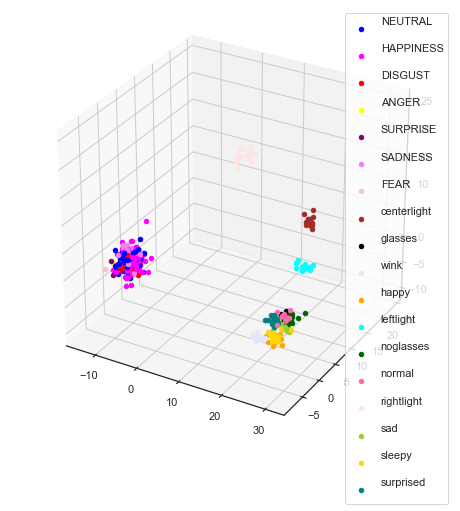
\includegraphics[width=16cm]{Scatter_Plot_of_lda.png}
	\caption{Scatter Plot of LDA Features}
	%	\label{fig:verticalcell}
\end{figure}

	\begin{figure}[H]
	\centering
	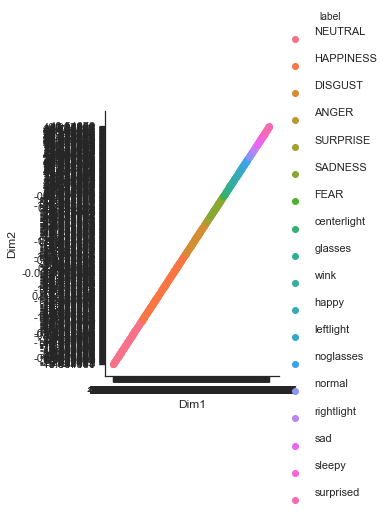
\includegraphics[width=16cm]{Emotion_Classification_TSNE.png}
	\caption{Facetgrid plot TSNE features}
	\label{fig:verticalcell}
\end{figure}


\end{problem}





\pagebreak

\end{document}
